\documentclass[12pt,a4paper]{article}
\usepackage[top=25.4mm, bottom=25.4mm, left=19.1mm, right=19.1mm]{geometry}


\usepackage[latin2]{inputenc}
\usepackage{graphicx}
\graphicspath{ {./images/} }
\usepackage{ulem}
\usepackage{amsmath}
\usepackage[document]{ragged2e}

\setlength{\parindent}{4em}
\setlength{\parskip}{1em}
\usepackage{hyperref}

\usepackage{fancyhdr}
\pagestyle{fancy}
\fancyhf{}
\fancyhead[LO]{\textbf{\small IoT and Smart Analytics}\\
\text{\small A Program by IIITH and TalentSprint}}

\usepackage{xcolor}
\usepackage{lipsum}

\rhead{\begin{picture}(0,0) \put(-250,-2){
\includegraphics[width=9cm]{EXP_08_Images/ts-iisc-logo-pr.png}} \end{picture}}
\cfoot{\thepage}


\begin{document}

\begin{center}

\textbf{\large \\EXPERIMENT 13 }\\[6pt]
Interfacing HC-SR04 Ultrasonic Sensor,
Single Channel Relay, and HC-SR501 PIR Motion Sensor with Arduino
\end{center}

\textbf{\large LEARNING OBJECTIVES:}\\[3pt]
At the end of this experiment, participants will be able to:\vspace{-6mm}\begin{enumerate}
 \setlength\itemsep{-0.3em}
\item Understand \& use HC-SR04 Ultrasonic Sensor, Single Channel Relay, \& HC-SR501 PIR Motion Sensor
\item Interface all above components with the Arduino
\end{enumerate}
\textbf{\large APPARATUS REQUIRED:}\\
\vspace{-0.1mm}
\begin{enumerate}
 \setlength\itemsep{-0.1em}
\item HC-SR04 Ultrasonic Sensor - 1pcs \\[3pt]
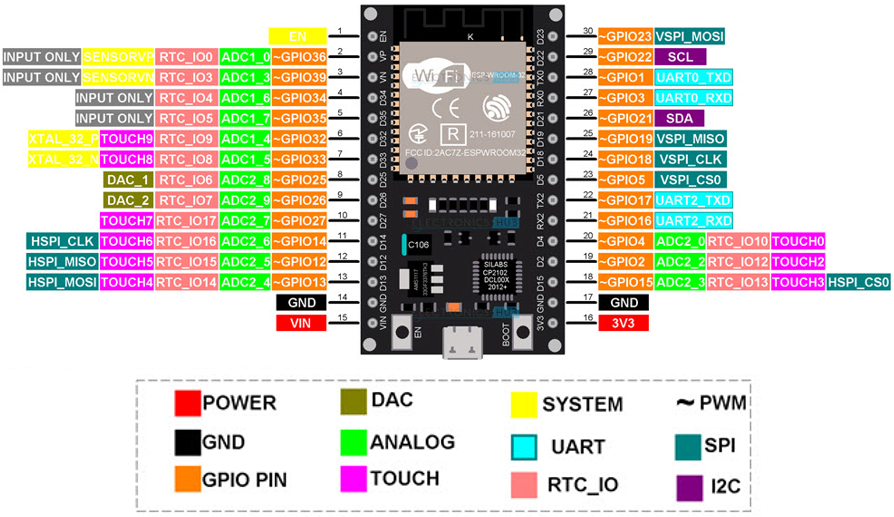
\includegraphics[scale=0.9]{EXP_13_Images/fig1.PNG}\\[3pt]
Figure 1. HC-SR04 Ultrasonic Sensor

\item HC-SR501 PIR Motion Sensor - 1pcs\\[3pt]
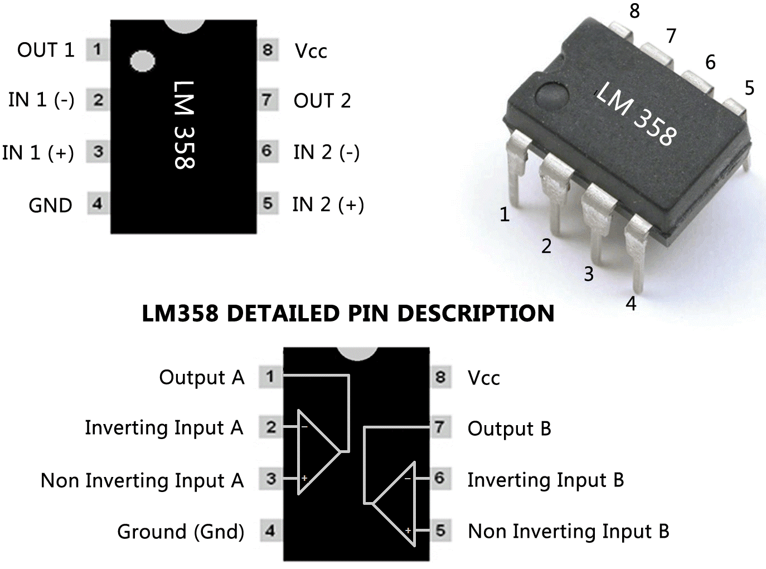
\includegraphics[scale=1.1]{EXP_13_Images/fig2.PNG}\\[3pt]
Figure 2. HC-SR501 PIR Motion Sensor

\item Single Channel Relay -1pcs\\[3pt]
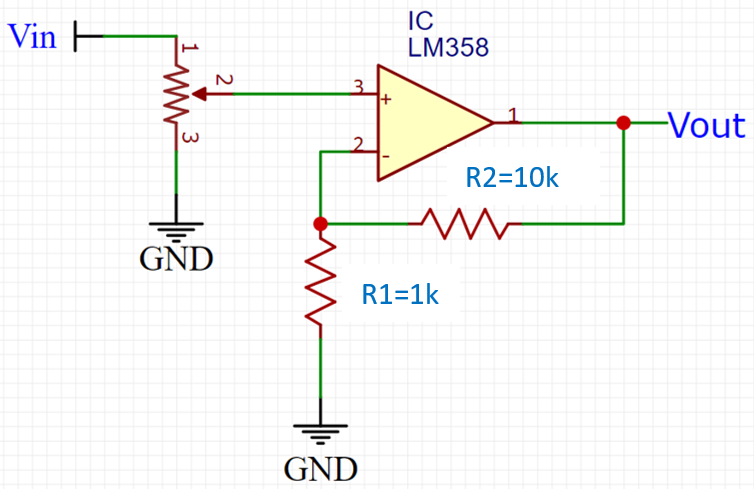
\includegraphics[scale=0.75]{EXP_13_Images/fig3.PNG}\\[3pt]
Figure 3. Single Channel Relay
\vspace{1cm}
\item Arduino  -1pcs\\
\item Breadboard -1pcs\\
\item LED -1pcs\\
\item Resistor 10 k$\Omega$ - 1pcs\\ 
\item Jumper wires\\
\end{enumerate}
\begin{justify}
\textbf{\large THEORY}\\[3pt]
\textbf{A)	HC-SR501 PIR Motion Sensor: } 
These sensors work on the principle of sensing Infrared waves to detect the motion of an object. PIR (Passive Infrared) sensor or PIR motion sensor is the kind of sensor that measures the Infrared radiations released from objects and thus identify them as moving or still objects. This type of motion sensor is only the receptor of infrared waves and does not release any infrared beam like that is done in Active Infrared sensors (AIR sensors).
\vspace{-6mm}
\begin{center} 
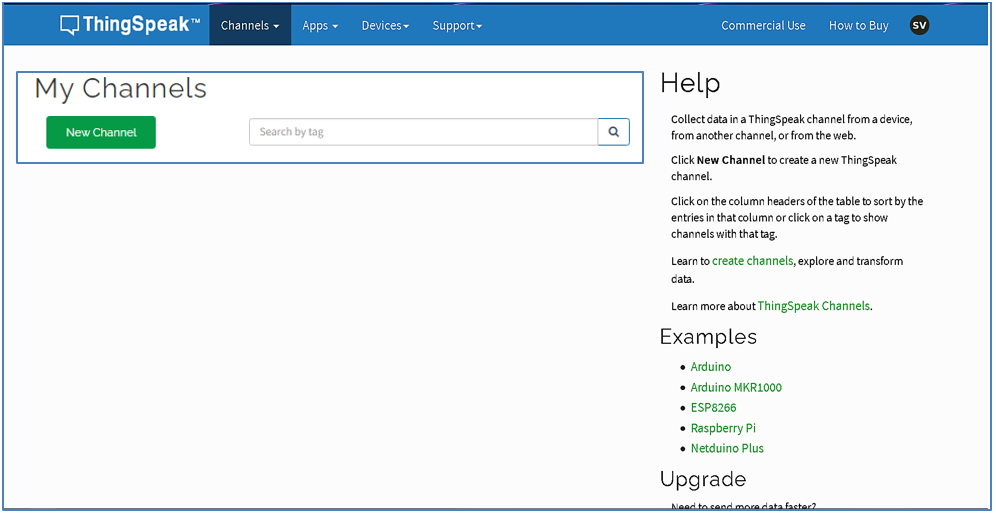
\includegraphics[scale=0.45]{EXP_13_Images/fig4.PNG}
\end{center}
\vspace{-10mm}
\begin{center} {Figure 4. Working of PIR Motion sensor: Heat source movement and output signal [1]}\end{center}
\vspace{-5mm}
\noindent The PIR sensor itself has two slots in it, each slot is made of a special material that is sensitive to IR as shown in fig. 4 above. The lens used here is not doing much and so we see that the two slots can 'see' out past some distance (basically the sensitivity of the sensor). When the sensor is idle, both slots detect the same amount of IR, the ambient amount radiated from the room or walls or outdoors. When a warm body like a human or animal passes by, it first intercepts one-half of the PIR sensor, which causes a positive differential change between the two halves. When the warm body leaves the sensing area, the reverse happens, whereby the sensor generates a negative differential change. These change pulses (as shown in the 'Output signal' of fig.4) are what is detected.
\vspace{-5mm}
\begin{center} 
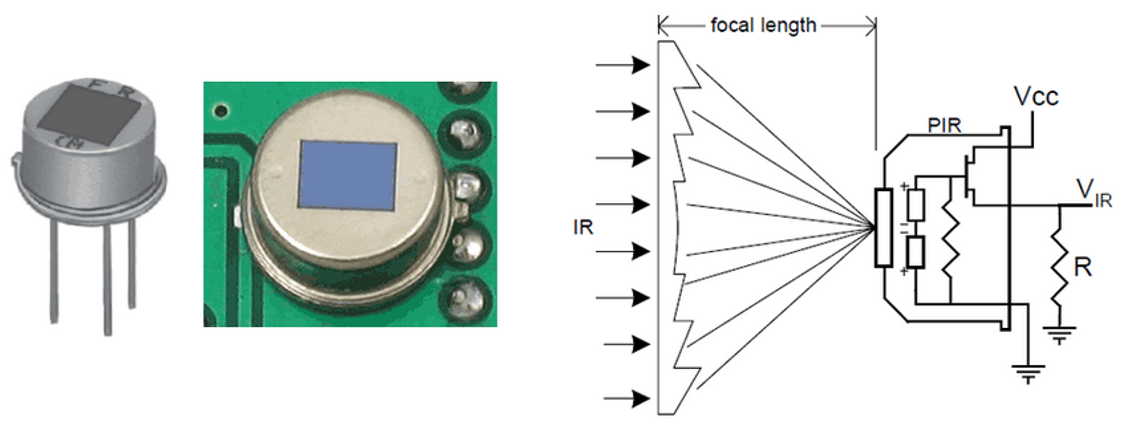
\includegraphics[scale=0.45]{EXP_13_Images/fig5.PNG}
\end{center}
\vspace{-5mm}
\begin{center} {Figure 5. The housing of IR sensor and Fresnel lens [1]}\end{center}

\noindent The IR sensor itself is housed in a hermetically sealed metal can shown in fig.5, to improve noise/temperature/humidity immunity. There is a window made of IR-transmissive material (typically coated silicon since that is very easy to come by) that protects the sensing element. Behind the window are the two balanced sensors. The Fresnel lens, used to cover the IR sensor, condenses light, providing a larger range of IR to the sensor.\par
\noindent There are also two potentiometers and a jumper on the HC-SR501 PIR Motion Sensor board, shown in fig.6, to adjust a couple of parameters:
\vspace{-3mm}
\begin{itemize}
\setlength\itemsep{-0.3em}
\item \textbf{SENSITIVITY} - This sets the maximum distance that motion can be detected. It ranges from 3 meters to approximately 7 meters. 
\item \textbf{TIME} -  This sets how long that the output will remain HIGH after detection. At minimum it is 3 seconds, at maximum, it is 300 seconds or 5 minutes.\\[6pt]
The jumper on the board has two settings:
\item \textbf{H} - This is the Hold or Repeat setting. In this position, the HC-SR501 will continue to output a HIGH signal as long as it continues to detect movement.
\item \textbf{L} - This is the Intermittent or No-Repeat setting. In this position, the output will stay HIGH for the period set by the TIME potentiometer adjustment
\end{itemize}
\vspace{-6mm}
\begin{center} 
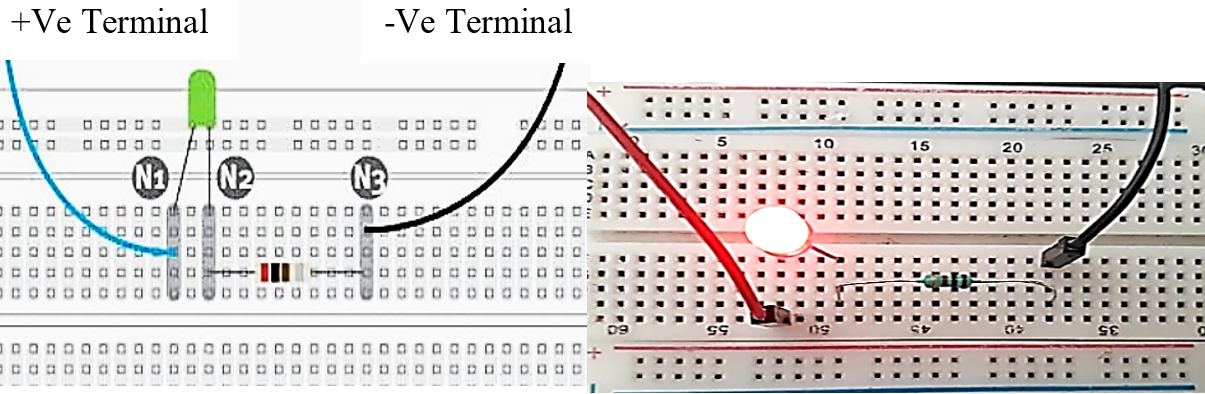
\includegraphics[scale=0.5]{EXP_13_Images/fig6.PNG}
\end{center}
\vspace{-5mm}
\begin{center} {Figure 6. Potentiometer and Jumper in HC-SR501 PIR sensor \& Pinouts}\end{center}


\noindent \textbf{B) HC-SR04 Ultrasonic Sensor: } Ultrasonic distance sensors use pulses of ultrasonic sound (sound above the range of human hearing) to detect the distance between them and nearby solid objects. The sensors consist of two main components shown in fig. :
\vspace{-4mm}
   \begin{itemize}
   \setlength\itemsep{-0.3em}
    \item \textbf{An Ultrasonic Transmitter} - This transmits the ultrasonic sound pulses, it operates at 40 kHz.
    \item \textbf{An Ultrasonic Receiver} - The receiver listens for the transmitted pulses. If it receives them it produces an output pulse whose width can be used to determine the distance the pulse traveled.\\[6pt] 
    The HC-SR04 has the following four connections:
    \item \textbf{VCC} - This is the 5 Volt positive power supply.
    \item \textbf{Trig} - This is the "Trigger" pin, the one driven to send the ultrasonic pulses.
    \item \textbf{Echo} - This is the pin that produces a pulse when the reflected signal is received. The length of the pulse is proportional to the time it took for the transmitted signal to be detected.
   \item \textbf{GND} - This is the Ground pin.
   \end{itemize}

\begin{center} 

\includegraphics[scale=0.6]{EXP_13_Images/fig7.PNG}
\end{center}
\begin{center} {Figure 7. Transmitter \& Receiver of an Ultrasonic Sensor [2]}\end{center}

\noindent The device operates as follows:

\begin{enumerate}
\setlength\itemsep{-0.3em}
    \item A 5-volt pulse of at least 10 $\mu$ S (10 microseconds) in duration is applied to the Trigger pin. 
    \item  The HC-SR04 responds by transmitting a burst of eight pulses at 40 kHz, shown in fig. 8. This 8-pulse pattern makes the "ultrasonic signature" from the device unique, allowing the receiver to discriminate between the transmitted pattern and the ultrasonic background noise.
    \item  The eight ultrasonic pulses travel through the air away from the transmitter. Meanwhile, the Echo pin goes high to start forming the beginning of the echo-back signal.
    \item  If the pulse is NOT reflected then the Echo signal will timeout after 38 mS (38 milliseconds) and return low. This produces a 38 mS pulse that indicates no obstruction within the range of the sensor.
    \item  If the pulse is reflected the Echo pin goes low when the signal is received.  This produces a pulse whose width varies between 150 $\mu$ S to 25 mS, depending upon the time it took for the signal to be received. The pulse trains are shown in fig. 8.
    \item The width of the received pulse is used to calculate the distance to the reflected object. Remember that the pulse indicates the time it took for the signal to be sent out and reflected back so to get the distance we need to divide the result in half. At sea level at 20° C sound travels at 343 m/s which is used for the value of the speed of sound. The width/duration of the received pulse is measured in micro-seconds while implemented in the Arduino code. The distance can be calculated as given below:
    
    Distance = (Speed of sound $\times$ Duration (Time))/2  \\[3pt]
    
     =  \text{ \large $ \frac{342X100 (cm)\times Duration(\mu S)}{1\times1000000(\mu S)} \times \frac{1}{2}$ }\\[3pt]
     
     = \text{ \large $\frac{Duration}{29.2}\  \times    \frac{1}{2}\ cm $}\\[3pt]
     
     = \text{ \large $\frac{Duration}{58.4}\ cm $}
\end{enumerate}
\vspace{2mm}
\begin{center} 

\includegraphics[scale=0.65]{EXP_13_Images/fig8.PNG}
\end{center}
\begin{center} {Figure 8. Transmitted/received pulse train and signal at Echo pin [3]}\end{center}

\begin{center} 
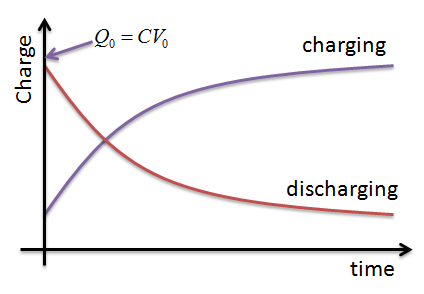
\includegraphics[scale=0.5]{EXP_13_Images/fig9.PNG}
\end{center}
\begin{center} {Figure 9. Pinouts of HC-SR04 Ultrasonic Sensor}\end{center}

\noindent \textbf{C) Single Channel Relay:} Relay is an electro-mechanical device that acts as a switch. DC electrical current is used to energize the relay coil which opens or closes the contact switches. The internal circuit of a single channel 5V relay consists of normally open contacts, normally closed contacts, and a coil. The figure below shows a pinout diagram of a single channel relay i.e. having only one relay inside.


\begin{center} 
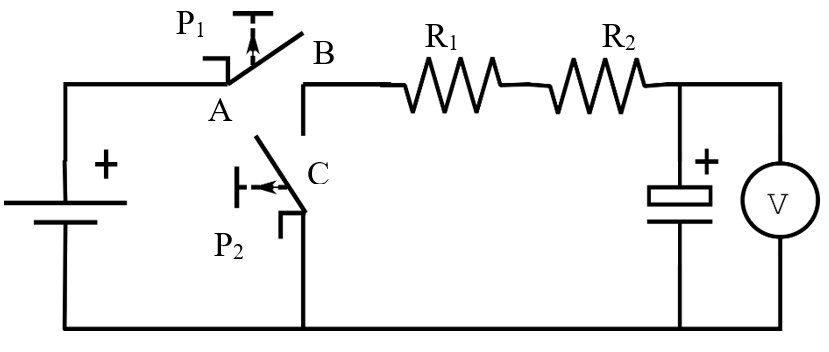
\includegraphics[scale=0.5]{EXP_13_Images/fig10.PNG}
\end{center}
\begin{center} {Figure 10. Relay pinouts}\end{center}

\noindent The following circuit shows the internal circuit diagram of a 5V single channel relay module. As we can see, on passing a high signal to the input pin of the relay, the NPN transistor starts conducting current between terminals 2, and 3 and the relay gets activated.

\begin{center} 
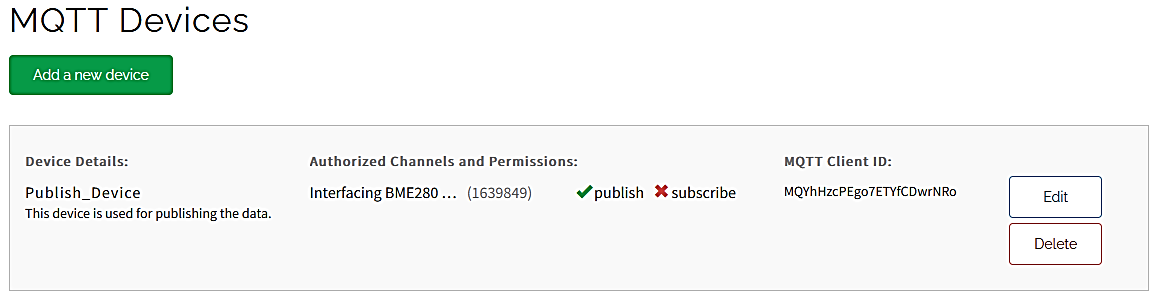
\includegraphics[scale=0.65]{EXP_13_Images/fig11.PNG}
\end{center}
\begin{center} {Figure 11. Internal circuit diagram of a single channel relay [4]}\end{center}

\noindent \textbf{\large PROCEDURE}\\[3pt]
\textbf{A) Interfacing HC-SR04 Ultrasonic Sensor \& Relay with Arduino }\\[3pt]
\textbf{Hardware and software setup :} The 'Echo' \& 'Trig' pins of the sensor module are connected to pins 10 \& 9 of the Arduino as shown in fig. 12 below. The input signal to the relay is supplied through the 'In' pin that is connected to the Pin 7 of the Arduino which is also connected to the anode of the LED via a resistor. In this example whenever an object is at a distance of 10 cm or less the LED will glow and the relay is triggered simultaneously. The distance of the object is also read in the serial monitor. The code is given below with commented explanation..\end{justify}

\begin{center} 
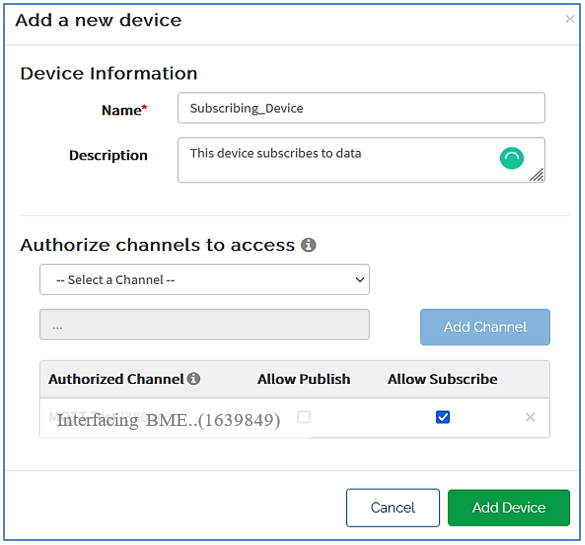
\includegraphics[scale=0.65]{EXP_13_Images/fig12.PNG}
\end{center}
\vspace{-5mm}
\begin{center} {Figure 12. Connection diagram for Ultrasonic sensor, Relay \& Arduino}\end{center}
\vspace{-5mm}
\hspace{1.5cm}\textbf{\large Code:}\\[6pt]
\setlength{\parindent}{8eM}


\textcolor{blue}{/* - Connect Gnd pin of the sensor to GND of Arduino\\
    - Connect Vcc of sensor to the 5v of Arduino*/}\\
int trigPin = 9;\textcolor{blue}{ // connect trig pin of sensor to pin 9 of Arduino}\\
int echoPin = 10;  \textcolor{blue}{// connect echo pin of sensor to pin 10 of Arduino}\\
int led = 7; \textcolor{blue}{ // connect positive end of LED to pin 7 of Arduino}\\
\textcolor{blue}{/* - Connect IN pin of relay to the same pin 7 of Arduino through \\  breadboard\\
    - Connect Vcc of the relay to the 5v of Arduino\\
    - Connect the GND of Relay to GND of Arduino */}\\[6pt]
void setup()\\
\{\\
   Serial.begin(9600); \\
   pinMode(led, OUTPUT);\\
   pinMode(trigPin, OUTPUT);\\
   pinMode(echoPin, INPUT);\\
  \textcolor{blue}{// put your setup code here, to run once:}\\
 \}\\[6pt]

void loop()\\ 
\{\\
  long duration, distance;\\
  digitalWrite(trigPin,HIGH);\\
  delayMicroseconds(10);\\
  digitalWrite(trigPin, LOW);\\
  duration=pulseIn(echoPin, HIGH); \textcolor{blue}{//See the ref.[5]}\\
  distance = duration/58.4;\\
  Serial.print(distance);\\
  Serial.println("CM");\\
  delay(1000);\\
 
    if (distanc $ <= $ 10 ) \\
       \{\\
       digitalWrite(led, HIGH);\\
        \}\\
    else if (distance $>$ 10) \\
       \{\\
     digitalWrite(led, LOW);\\
       \}\\
  \}\\

\vspace{5mm}

\setlength{\parindent}{0pt}
\textbf{B) Interfacing HC-SR501 PIR Motion Sensor with Arduino }\\[3pt]
\textbf{Hardware and software setup :}The output pin of the sensor module (middle pin) is connected to pin 2 of the Arduino and an LED is connected to pin 13 of the Arduino via a resistor as shown in fig. 13 below. Whenever a motion is detected in the vicinity of the sensor the LED will glow and a message is displayed in the serial monitor. The code with commented explanation is given below.
\vspace{-5mm}
\begin{center} 
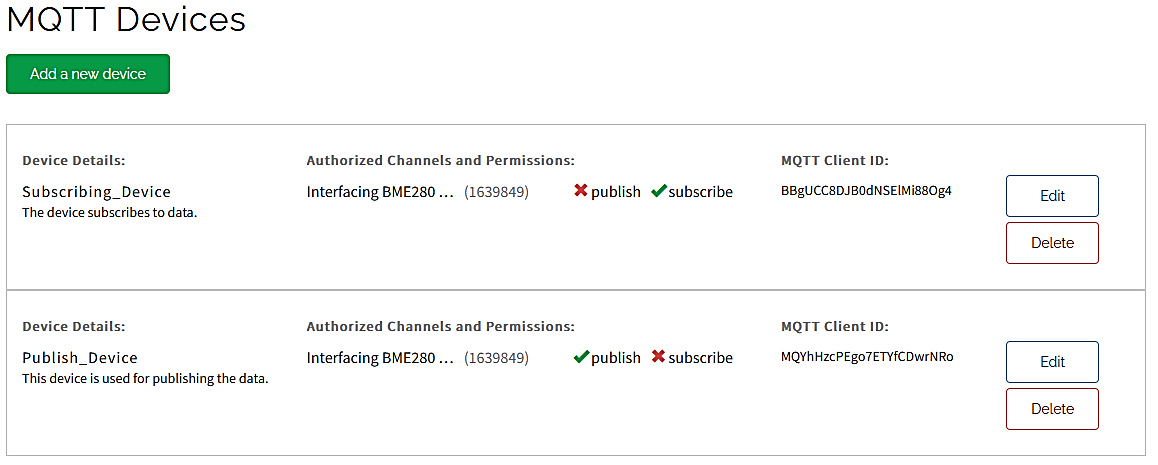
\includegraphics[scale=0.9]{EXP_13_Images/fig13.PNG}
\end{center}
\vspace{-5mm}
\begin{center} {Figure 13. Connection diagram for PIR Sensor \& Arduino}\end{center}


\hspace{1.5cm}\textbf{\large Code:}\\[6pt]
\setlength{\parindent}{8eM}

int led = 13;    \textcolor{blue}{// the pin that the LED is attached to}\\
int sensor = 2;\textcolor{blue}{// the pin that the sensor is atteched to}\\
int state = LOW;\textcolor{blue}{// by default, no motion detected}\\
int val = 0;  \textcolor{blue}{// variable to store the sensor status (value)}\\[6pt]

void setup()\\
\{\\
  pinMode(led, OUTPUT); \textcolor{blue}{// initalize LED as an output}\\
  pinMode(sensor, INPUT);\textcolor{blue}{// initialize sensor as an input}\\
  Serial.begin(9600); \textcolor{blue}{// initialize serial}
  \}\\[6pt]

void loop()\\
\{\\
  val = digitalRead(sensor);\textcolor{blue}{// read sensor value}\\
  if (val == HIGH) \{ \textcolor{blue}{ // check if the sensor is HIGH}\\
    digitalWrite(led,HIGH);\textcolor{blue}{// turn LED ON}\\
    delay(100);  \textcolor{blue}{// delay 100 milliseconds }\\
    
     if (state == LOW) \\
     \{\\
         Serial.println("Motion detected!"); \\
         state = HIGH; \textcolor{blue}\\
         \}\\
    \}\\ 
  else \\
  \{\\
       digitalWrite(led,LOW);\textcolor{blue}{ // turn LED OFF}\\
       delay(200); \textcolor{blue}{// delay 200 milliseconds}
      
         if (state == HIGH)\\
         \{\\
         Serial.println("Motion stopped!");\\
        state = LOW;  \textcolor{blue}{// update variable state to LOW}\\
          \}\\
      \}\\
  \}\\



\setlength{\parindent}{0eM}
\begin{justify}

\noindent \textbf{\large REFERENCES:}
\vspace{-3mm}
\begin{enumerate}
 \setlength\itemsep{-0.3em}
\item \href{https://learn.adafruit.com/pir-passive-infrared-proximity-motion-sensor/how-pirs-work}{Working of PIR Motion Sensor}
\item \href{https://medium.com/@aquibansari12377/ultrasonic-sensor-and-arduino-tutorial-89c38c81f103}{Ultrasonic Sensor}
\item \href{https://datasheetspdf.com/pdf-file/1380138/ETC1/HC-SR04/1}{Datasheet of  HC-SR04}
\item \href{https://components101.com/switches/5v-single-channel-relay-module-pinout-features-applications-working-datasheet}{Internal Circuit Diagram for Single Channel Relay Module}
\item \href{https://www.arduino.cc/en/Reference.PulseIn}{'pulseIn' function in Arduino}
\item \href{https://cdn-learn.adafruit.com/downloads/pdf/pir-passive-infrared-proximity-motion-sensor.pdf}{Datasheet of HC-SR501 PIR Motion Sensor}
\end{enumerate}

\noindent \textbf{\large CONCEPT DRILLS}\\[3pt]
Design a circuit and write the appropriate program in Arduino so that whenever a motion is detected by the PIR sensor a relay gets triggered.

\end{justify}
\end{document}